\section{Grundlegendes der Mechanik}

\subsection{Newtonsche Gesetze}

Gesetze, welche Bewegungen beschreiben. Oftmals ein Skalar und dessen Einfluss mit einer vektoriellen Grösse.


\subsubsection{Erstes Newtonsches Gesetz: Trägheitsgesetz}

Ein Körper verharrt in seine Zustand (Ruhe, gleichförmige geradlinige Bewegung), wenn er nicht durch eine Kraft gezwungen wird, 
seinen Zustand zu ändern.

Die \textbf{Trägheit} eines Körpers hängt von seiner (Trägheits-) Masse ab.


\subsubsection{Zweites Newtonsches Gesetz: Aktionsgesetz}

\begin{minipage}{0.2\columnwidth}
	$$ \boxed {\vec{F} = m \cdot \vec{a} } $$
\end{minipage}
\hfill
\begin{minipage}{0.75\columnwidth}
	\begin{tabular}{c l c}
		$\vec{F}$ 	& Kraft 				& $[F] = \frac{\kilo \gram \cdot \meter}{\second^2}  = \newton$ \\
		$m$ 		& (Trägheits-) Masse 	& $[m] = \kilo \gram$ 											\\	
		$\vec{a}$	&  Beschleunigung 		& $[a] = \frac{\meter}{\second^2}$
	\end{tabular}
\end{minipage}

\vspace{0.2cm}
\textrightarrow\ Anwendung erfolgt meist komponentenweise! \\

\begin{minipage}{0.2\columnwidth}
	$$ \boxed {\vec{F} = \frac{dp}{dt} \rightarrow \vec{F} = m \cdot \dot{v} + \dot{m} \cdot v} $$
\end{minipage}

\vspace{0.2cm}

\begin{minipage}{0.5\columnwidth}
	\begin{tabular}{c l c}
		$\vec{F}$ & Kraft                                       & $[F] = \frac{\kilo \gram \cdot \meter}{\second^2}  = \newton$ \\
		   $m$    & (Trägheits-) Masse                          & $[m] = \kilo \gram$                                           \\
		   $m$    & (Trägheits-) Masse abgeleitet nach der Zeit & $[m] = \frac{\kilo \gram}{\second}$                           \\
		   $v$    & Geschwindigkeit                             & $[v] = \frac{\meter}{\second}$                                \\
		   $v$    & Geschwindigkeit  abgeleitet nach der Zeit    & $[v] = \frac{\meter}{\second^2}$
	\end{tabular}
\end{minipage}


\subsubsection{Drittes Newtonsches Gesetz: Wechselwirkungsgesetz}

Wirkt ein Körper $A$ auf einen Körper $B$ mit der Kraft $\vec{F}_{\rm AB}$, so wirkt der Körper $B$ auf $A$ mit der
Kraft $\vec{F}_{\rm BA} = - \vec{F}_{\rm AB}$


\subsection{Reibungskräfte}

\begin{minipage}{0.37\columnwidth}
	$$ \boxed{ \text{Haften:} \quad \vec{F}_{\rm Rmax} = \mu_H \cdot \vec{F}_N } $$ 
\end{minipage}
\hfill
\begin{minipage}{0.37\columnwidth}
	$$ \boxed{ \text{Gleiten:} \quad \vec{F}_{\rm Rgleit} \approx \mu_G \cdot \vec{F}_N } $$ 
\end{minipage}
\hfill
\begin{minipage}{0.2\columnwidth}
	$$ \boxed{ \vert \vec{F}_R \vert \leq \vert \vec{F}_{\rm Rmax} \vert } $$
\end{minipage}

\vspace{0.2cm}

\begin{tabular}{lll}
	$\vec{F}_R$ 			& Reibungskraft 		& $[\vec{F}_R] = \newton$ 			\\
	$\vec{F}_{\rm Rmax}$ 	& Haftreibungskraft 	& $[\vec{F}_{\rm Rmax}] = \newton$ 	\\
	$\vec{F}_{\rm Rgleit}$ 	& Gleitreibungskraft 	& $[\vec{F}_{\rm Rgleit}] = \newton$
\end{tabular}


\subsection[Rollreibungslänge]{Rollreibungslänge $e$ (Drehmoment)}

\begin{minipage}{0.4\columnwidth}
	\begin{center}
		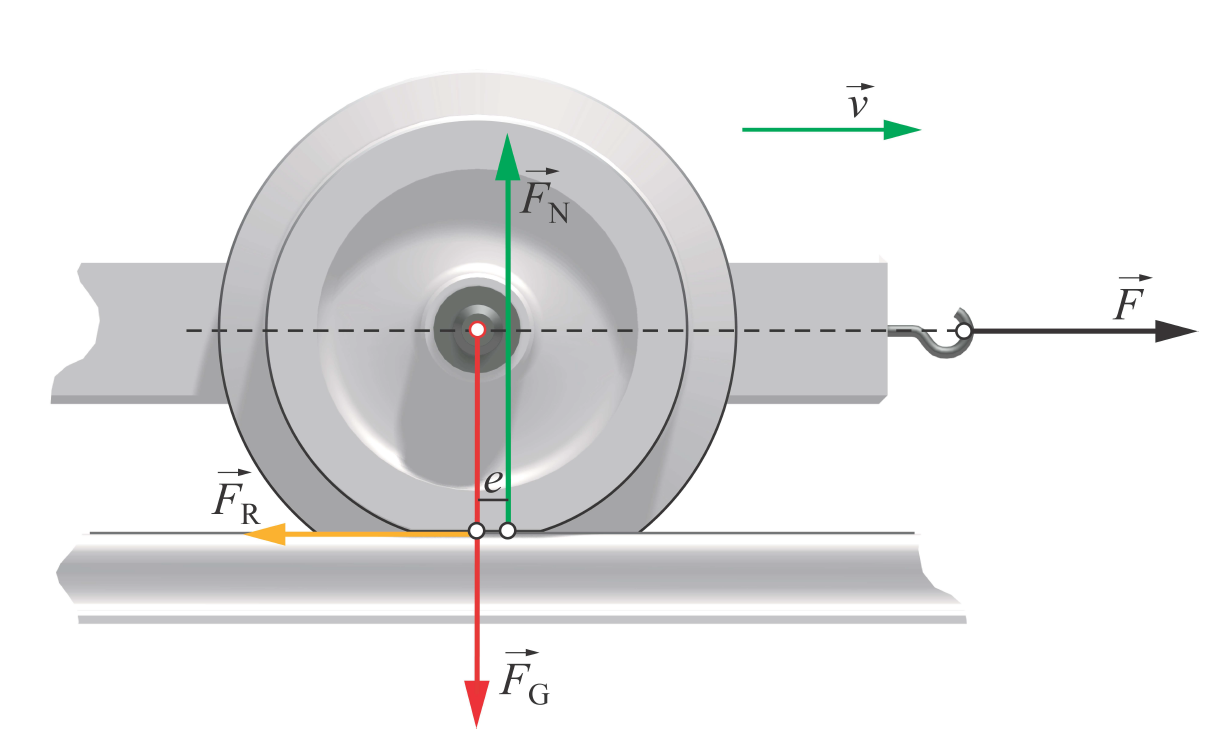
\includegraphics[width=\columnwidth]{images/rollreibung_1}
	\end{center}
\end{minipage}
\hfill
\begin{minipage}{0.48\columnwidth}
	\begin{center}
		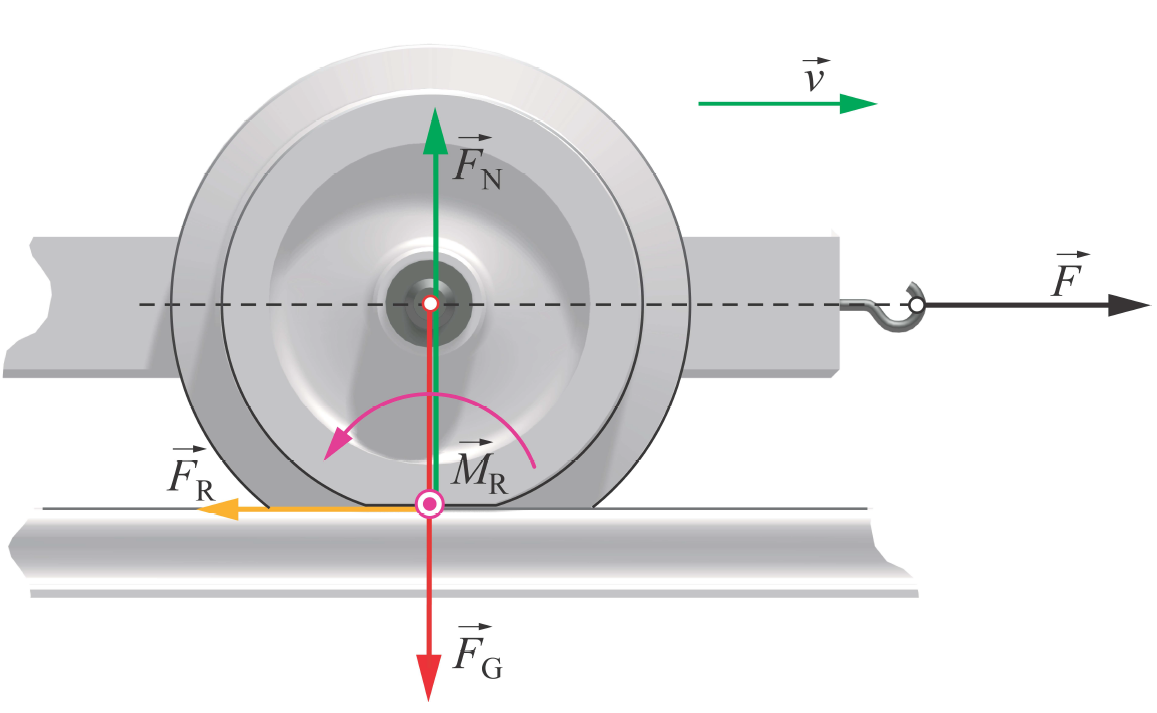
\includegraphics[width=\columnwidth]{images/rollreibung_2}
	\end{center}
\end{minipage}

$$ \boxed{ e = \frac{r \cdot F}{F_N} = \frac{r \cdot F_R}{F_N} =  \frac{r \cdot \mu_R \cdot F_R}{F_N} = \mu_R \cdot r }$$ 
$$ \boxed{ M_R = e \cdot F_N = \mu_R \cdot r \cdot F_N = r \cdot F_R = r \cdot F} $$


\begin{tabular}{c l c}
	$e$ 	& Rollreibungslänge 		& $[e] = \meter$ 			\\
	$r$ 	& Radius des Rades 			& $[r] = \meter$			\\
	$F_R$ 	& Rollreibungskraft 		& $[F_R] = \newton$ 		\\
	$F_N$ 	& Normalkraft 				& $[F_N] = \newton$ 		\\
	$\mu_R$ & Rollreibungskoeffizient 	& $[\mu_R] = 1$ 			\\
	$M_R$ 	& Rollreibungsmoment 		& $[M_R] = \newton \meter$
\end{tabular}


\subsection{Angetriebenes Rad}

\begin{center}
	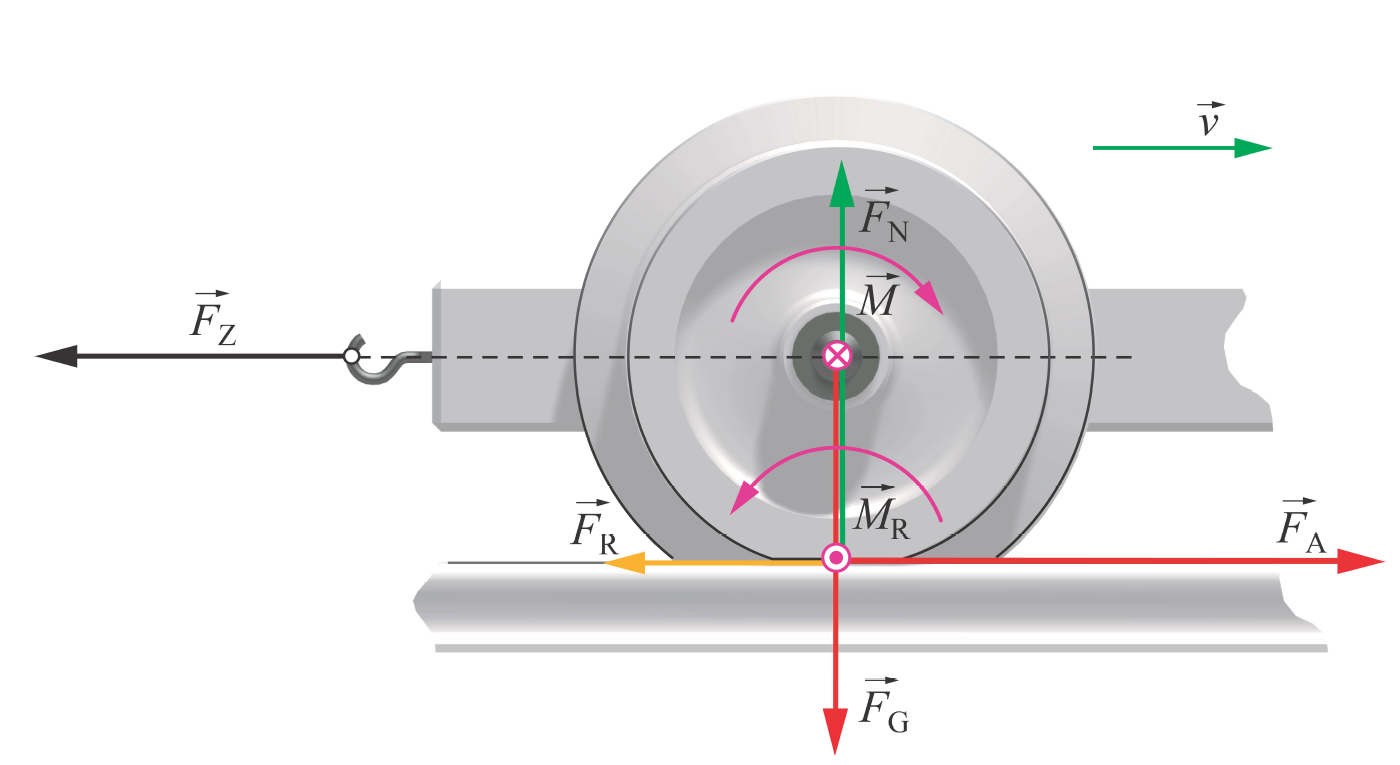
\includegraphics[width=0.8\columnwidth]{images/antriebsrad}
\end{center}

\vspace{0.2cm}
\begin{tabular}{c l c}
	$\vec{F_Z}$ & Zugkraft 			& $[F_Z] = \newton$ \\
	$\vec{F_N}$ & Normalkraft 		& $[F_N] = \newton$ \\
	$\vec{F_R}$ & Rollreibungskraft & $[F_R] = \newton$ \\
	$\vec{F_A}$ & Haftreibungskraft & $[F_A] = \newton$
\end{tabular}


\subsubsection{Hinweise zu Reibung an Rädern}

\begin{itemize}
	\item Jedes Rad weist Rollreibung auf
	\item Zusätzlich zur Rollreibung weist ein angetriebenes Rad eine Haftreibung auf
\end{itemize}


\subsection{Arbeit}

Wird der Angriffspunkt einer Kraft $\vec{F}$ um die Strecke $\diff \vec{s}$ verschoben so leistet die Kraft die Arbeit $W$ 
$$ \boxed{ W_{AB} =  \int \limits_A^B d \, W =  \int \limits_A^B \vec{F} \bullet d \, \vec{s} \qquad \text{(Skalarprodukt)} }$$
$$ \boxed{ \text{Wenn die projizierte Kraft konstant ist:} \quad  W = F \bullet s_{AB} } $$

\begin{tabular}{c l c}
	$W$ & Arbeit	& $[W] = \newton \cdot \meter = \joule$	\\
	$F$ & Kraft 	& $[F] = \newton$ 						\\
	$s$ & Weg 		& $[s] = \meter$ 						\\
\end{tabular}


\subsection{Energie}

\subsubsection{Potentielle Energie $W_{\rm pot}$}

Beim Anheben eines Körpers gewinnt der Körper an potentieller Energie (Lageenergie) 

$$ \boxed{ W_{\rm pot} = m \cdot g \cdot h} $$

\begin{tabular}{c l c}
	$W_{\rm pot}$ 	& Potentielle Energie	& $[W] = \newton \cdot \meter = \joule$ \\
	$m$ 			& Masse des Körpers 	& $[m] = \kilo \gram$ 					\\
	$g$ 			& Erdbeschleunigung 	& $[g] = \frac{\meter}{\second^2}$ 		\\
	$h$ 			& Höhe der Körpers 		& $[h] = \meter$
\end{tabular}


\example{Spannen einer Feder}

Federkraft als Funktion der Auslenkung $x$ \qquad $F = -k \cdot x$ 
$$ \boxed{ W_{\rm pot} = \int \limits_0^{x_0}  - \vec{F} \bullet d \vec{x} = \int \limits_0^{x_0}  k \cdot x \, dx = \frac{1}{2} \, k \cdot x_0^2} $$

\begin{tabular}{c l c}
	$W_{\rm pot}$ 	& Potentielle Energie 	& $[W] = \newton \cdot \meter = \joule$ \\
	$F$ 			& Federkraft 			& $[F] = \newton$ 						\\
	$k$ 			& Federkonstante 		& $[k] = \frac{\newton}{\meter}$ 		\\
	$x_0$ 			& Auslenkung der Feder 	& $[x_0] = \meter$	
\end{tabular}


\subsubsection{Kinetische Energie $W_{\rm kin}$}

$$ \boxed{ W_{\rm kin} = \int \limits_A^B \vec{F} \bullet d \, \vec{s} =  F \bullet s_{AB} = m \, a \cdot \frac{a}{2} t^2 = m \frac{a^2 \cdot t^2}{2} = \frac{1}{2} m \cdot v^2} $$


\begin{tabular}{c l c}
	$W_{\rm kin}$ 	& Kinetische Energi			 	& $[W] = \newton \cdot \meter = \joule$ \\
	$F$ 			& Kraft 						& $[F] = \newton$ 						\\
	$s$ 			& Wegstück (Kinematik) 			& $[s] = \meter$ 						\\
	$m$ 			& Masse des Körpers 			& $[m] = \kilo \gram$ 					\\
	$a$ 			& Beschleunigung (Kinematik) 	& $[a] = \frac{\meter}{\second^2}$ 		\\
	$v$ 			& Geschwindigkeit (Kinematik) 	& $[v] = \frac{\meter}{\second}$
\end{tabular}


\subsection{Energieerhaltung (in abgeschlossenen Systemen)}

Die Gesamtenergie eines \myul{abgeschlossenen Systems} ist unveränderlich! 

\textbf{abgeschlossen: Es wird keine Masse hinzugefügt/entfernt und es wirken keine äusseren Kräfte!} 
$$ \boxed{ W = \underbrace{m \cdot g \cdot h}_{\substack{\text{pot. Energie}}} 
	=  m \cdot g \cdot \underbrace{ \frac{1}{2} \, g \cdot t^2}_{\substack{\text{h(t)}}} 
	= \underbrace{ \frac{1}{2} m \cdot v^2 }_{\substack{\text{kin. Energie}}} } $$

Für \myul{nicht abgeschlossene Systeme} kann eine Bilanzrechnung aufgestellt werden:
\vspace{0.1cm}
\begin{itemize}
	\item Die Energiezunahme im Gesamtsystem entspricht der von aussen zugeführten Energie.
	\item Die Energieabnahme im Gesamtsystem entspricht der von aussen entzogenen Energie.
\end{itemize}


\subsubsection{Energiesatz der Mechanik} 

\vspace{-0.2cm}
$$ \boxed{ E_{\rm pot} + E_{\rm kin} = E_{\rm tot} = \text{const} } \qquad \text{(gilt zu jedem Zeitpunkt)} $$


\subsection{Leistung}

\vspace{-0.2cm}
$$ \boxed{ P = \frac{\Delta W}{\Delta t} = \frac{\vec{F} \bullet \Delta \vec{s}}{\Delta t} 
	= \vec{F} \frac{\Delta \vec{s}}{\Delta t} = \vec{F} \bullet \vec{v} } $$ 

\begin{tabular}{c l c}
	$P$ 		& Leistung 			& $[P] = \watt = \frac{\joule}{\second}$	\\
	$\Delta W$ 	& geleistete Arbeit & $[W] = \joule$							\\
	$\Delta t$ 	& verstrichene Zeit & $[t] = \second$ 							\\
	$F$ 		& Kraft 			& $[F] = \newton$ 							\\
	$\Delta s$ 	& Wegstück 			& $[s] = \meter$ 
\end{tabular}


\subsubsection{Pferdestärken}

$$ 1 \; \mathrm{PS} = 75 \, \kilo \gram \cdot 9.81 \, \frac{\meter}{\second^2} \cdot 1 \, \frac{\meter}{\second} = 735.5 \, \watt $$


\subsection[Wirkungsgrad]{Wirkungsgrad $\eta$}	

Faustregel: Je grösser eine Maschine, desto besser ihr Wirkungsgrad 
$$ \boxed{ \eta = \frac{P_{\rm ab}}{P_{\rm zu}} } \qquad \cor{\eta < 1} \qquad [\eta] = 1 $$


\subsection[Impuls]{Impuls $\vec{p}$}

\vspace{-0.2cm}
$$ \boxed{ \vec{p} = m \cdot \vec{v} }$$ 

2. Newton'sches Gesetz allgemeingültiger (relativistisch):
$$ \boxed{ \vec{F} = m \cdot \vec{a} = m \cdot \frac{\diff \vec{v}}{\diff t} = \frac{\diff}{\diff t} (m \cdot \vec{v}) = \frac{\diff \vec{p}}{\diff t} } $$ 


\begin{tabular}{c l c}
	$\vec{p}$ 	& Impuls 			& $[\vec{p}] = \frac{\kilo \gram \, \meter}{second}$	\\
	$m$ 		& Masse 			& $[m] = \kilo \gram$ 									\\
	$\vec{v}$ 	& Geschwindigkeit 	& $[v] = \frac{\meter}{\second}$ 						\\
	$F$ 		& Kraft 			& $[F] = \newton$ 										\\
	$\vec{a}$ 	& Beschleunigung 	& $[\vec{a}] = \frac{\meter}{\second^2}$
\end{tabular}


\subsubsection{Kraftstoss $\Delta p$}

Ein Kraftstoss entspricht einer \textbf{Impulsänderung} und kann über die mittlere Kraft beschrieben werden. 

\begin{minipage}{0.55\columnwidth}
	$$ \boxed{ \int \limits_{t_a}^{t_a + \Delta t}  F(t) \, \diff t = \overline{F} \cdot \Delta t = \Delta p = p' - p } $$ 	
\end{minipage}
\hfill
\begin{minipage}{0.42\columnwidth}
	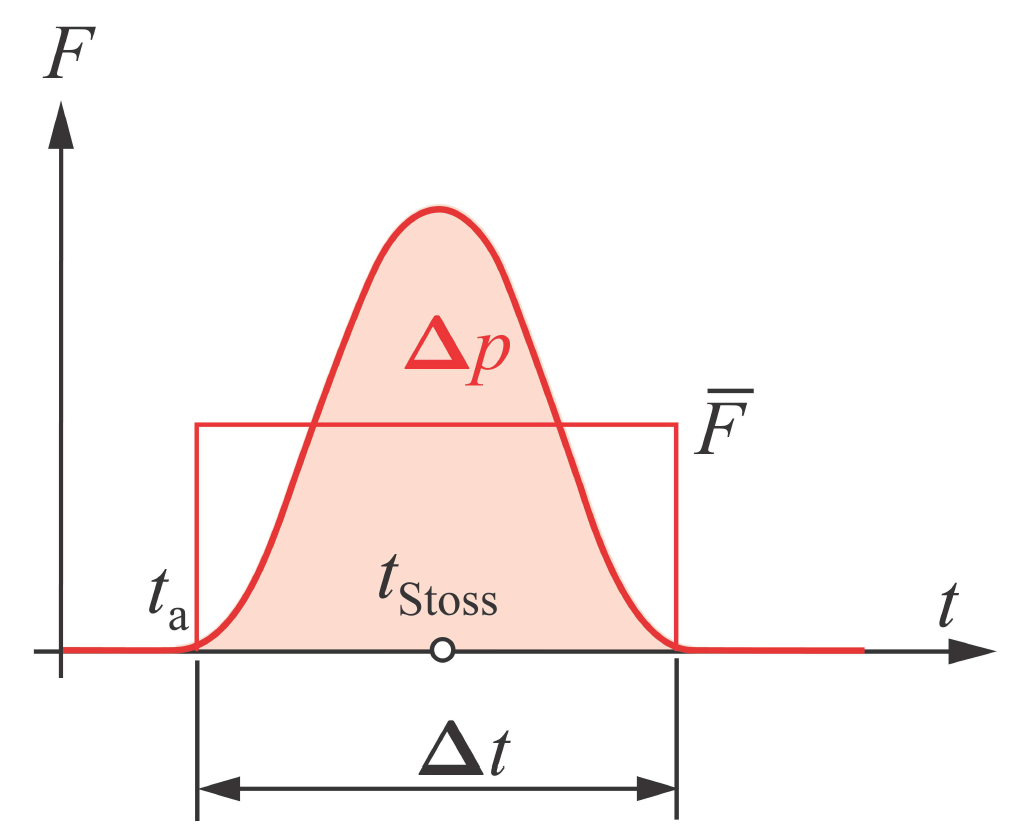
\includegraphics[width=0.8\columnwidth]{images/impuls}
\end{minipage}

\begin{tabular}{c l c}
	$F(t)$ 			& Kraftverlauf 					& $[F] = \newton$ 					\\
	$\overline{F}$ 	& mittlere Kraft 				& $[\overline{F}] = \newton$		\\
	$\Delta t$ 		& Zeitdauer des Kraftstosses	& $[\Delta t] = \second$ 			\\
	$\Delta p$ 		& Impulsänderung 				& $[\Delta p] = \newton \second$ 	\\
	$p$ 			& Impuls vor dem Stoss 			& $[p] = \newton \second$ 			\\
	$p'$ 			& Impuls nach dem Stoss 		& $[p'] = \newton \second$ 			\\
	$\vec{a}$ 		& Beschleunigung 				& $[\vec{a}] = \frac{\meter}{\second^2}$
\end{tabular}


\subsection{Impulserhaltungssatz (Impulssatz)}
In einem \textbf{abgschlossenen System} bleibt der \textbf{Gesamtimpuls konstant}
Abgeschlossenes System: es wirken keine externen Kräfte 
$$ \boxed{ \vec{p} =  \int \underbrace{ \frac{\diff \vec{p}}{\diff t} }_{\substack{F_{\rm aussen} = 0}}  \, \diff t = c = \text{const} }  $$


\subsection{Stösse}

\renewcommand{\arraystretch}{2}
\begin{tabular}{ll}
	Elastizitätszahl: 	& $k = \frac{v_2' - v_1'}{v_1 - v_2} = - \frac{v'_{rel}}{v_{rel}} \geq 0$ \\
	Deformtionsarbeit: 	& $Q = (E_1 + E_2) - (E_1' + E_2') \geq 0$ 
\end{tabular}
\renewcommand{\arraystretch}{1.3}

\vspace{0.2cm}
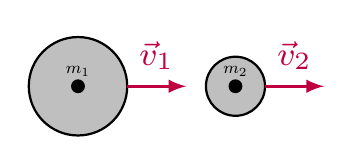
\begin{tikzpicture}
    [
    x=1cm, y=1cm, scale=0.5, font=\footnotesize, >=latex 
    %Voreinstellung für Pfeilspitzen
    ]
    %Raster im Hintergrund
    %\draw[step=1, gray, very thin] (0,0) grid (5.5,5.5);
    
    %m1
    \begin{scope}[xshift=0cm, yshift=0cm, rotate=0, scale=1]
        %Kräfte
        \fill[gray!50!white] (0, 0) circle(1.25);
        \draw[thick] (0, 0) circle(1.25);
        \fill[black] (0, 0) circle(5pt) node [midway, above, yshift=2pt, scale=1.5] {$m_1$};
        \draw [-latex, very thick, purple] (1.25,0) -- ++(1.5,0) node[midway, above, scale=1.5] {$\vec{v}_1$};
    \end{scope}		
    
    %m2
    \begin{scope}[xshift=4cm, yshift=0cm, rotate=0, scale=1]
        %Kräfte
        \fill[gray!50!white] (0, 0) circle(0.75);
        \draw[thick] (0, 0) circle(0.75);
        \fill[black] (0, 0) circle(5pt) node [midway, above, yshift=2pt, scale=1.5] {$m_2$};
        \draw [-latex, very thick, purple] (0.75,0) -- ++(1.5,0) node[midway, above, scale=1.5] {$\vec{v}_2$};
    \end{scope}	
\end{tikzpicture}



\subsubsection{Gerader, zentraler, total elastischer Stoss}


Die beiden Stosspartner verformen sich \textbf{nicht}!

\textrightarrow\ Für die Deformationsarbeit gilt: $Q = 0$

\vspace{0.2cm}

\boxed{
	\begin{tabular}{ll}
		Impulssatz: 	&  $p  \overset{!}{=} p'$ 																										\\
		& $m_1 \, v_1 + m_2 \, v_2 \overset{!}{=} m_1 \, v_1' + m_2 \, v_2'$ 															\\
		\\
		Energiesatz: 	& $E_{\rm kin} \overset{!}{=} E_{\rm kin}'$ 																					\\
		& $\frac{1}{2} m_1 \, v_1^2 + \frac{1}{2} m_2 \, v_2^2 \overset{!}{=} \frac{1}{2} m_1 \, v_1'^2 + \frac{1}{2} m_2 \, v_2'^2 $ 	\\
		\\
		& $v_1' = \frac{m_1 - m_2}{m_1 + m_2} \cdot v_1 + \frac{2 \, m}{m_1 + m_2} \cdot v_2$ 											\\
		\\
		& $v_2' = \frac{2 \, m_1}{m_1 + m_2} \cdot v_1 + \frac{m_2 - m_1}{m_1 + m_2} \cdot v_2$
	\end{tabular}
}


\subsubsection{Gerader, zentraler, total inelastischer Stoss}

Die beiden Stosspartner haften nach dem Stoss \textbf{aneinander} und haben die \textbf{gleiche Geschwindigkeit}.

\textrightarrow\ Für die Deformationsarbeit gilt: $Q \neq 0$

\vspace{0.2cm}

\boxed{
	\begin{tabular}{ll}
		Impulssatz: 			& $p  \overset{!}{=} p'$ 																		\\
		& $m_1 \, v_1 + m_2 \, v_2 \overset{!}{=} (m_1 + m_2) \, v'$ 									\\
		\\
		Energiesatz: 			& $E_{\rm kin} \overset{!}{=} E_{\rm kin}'$ 													\\
		& $\frac{1}{2} m_1 \, v_1^2 + \frac{1}{2} m_2 \, v_2^2 \overset{!}{=} \frac{1}{2} (m_1 + m_2) \, v'^2 + Q$ 				\\
		\\
		Deformationsarbeit: 	& $Q = \frac{m_1 \, m_2}{2 (m_1 + m_2)} (v_1 - v_2)^2 =  \frac{1}{2} \mu \cdot v_{\rm rel}^2 $ 	\\
		\\
		Relativgeschwindigkeit: & $v_{\rm rel} := \vert v_1 - v_2  \vert$ 														\\
		\\
		Reduzierte Masse: 		& $\mu = \frac{m_1 \, m_2}{m_1 + m_2}$
	\end{tabular}
}

\begin{tabular}{c l c}
	$k$ 			& Elastizitätszahl 				& $[k] = 1$ 							\\
	$E_1, \,E_2$ 	& Energien vor Stoss 			& $[E] = \joule$ 						\\	
	$E_1', \, E_2'$ & Energien nach Stoss	 		& $[E'] = \joule$ 						\\	
	$m_1, \, m_2$ 	& stossende Massen 				& $[m] = \kilo \gram$ 					\\
	$v_1, \, v_2$ 	& Geschwindigkeit vor Stoss 	& $[v] = \frac{\meter}{\second}$ 		\\
	$v_1', \, v_2'$ & Geschwindigkeit nach Stoss 	& $[v'] = \frac{\meter}{\second}$ 		\\
	$Q$ 			& Deformationsarbeit 			& $[Q] = \joule$ 						\\
	$v_{\rm rel}$ 	& Relativgeschwindigkeit 		& $[v_{rel}] = \frac{\meter}{\second}$ 	\\
	$\mu$ 			& Reduzierte Masse 				& $[\mu] = \kilo \gram$ 
\end{tabular}


\pagebreak